
\documentclass[a4paper,12pt]{scrbook}
\usepackage{amsmath,amssymb,amsthm}
\usepackage{fancyvrb}
\usepackage{parskip}
\usepackage{lastpage}
\usepackage{verbatim,boxedminipage,enumitem}
\usepackage{ifthen}
\usepackage{color,graphicx}
\usepackage{pgf}
\usepackage{longtable}
\usepackage{upquote}
%\usepackage[all]{xy}
\usepackage{tobiShell}
\usepackage{tikz}
\usetikzlibrary{automata}
\usetikzlibrary{arrows}
\usepackage{pgf,pgfarrows,pgfnodes}
\usepackage{pgfplots}
\usepackage{circuitikz}
\usetikzlibrary{circuits}
\usetikzlibrary{circuits.logic.US}
\usepackage{mymath}
\usepackage{python}
%------------------------------------------------------------------
% Verbatim for console window - single line frame, no line numbers
%------------------------------------------------------------------
\DefineVerbatimEnvironment%
 {console}{Verbatim}
 {frame=single}

%--------------------------------------------------------
% Remove the vertical spacing before and after Verbatim.
%--------------------------------------------------------
\usepackage{atbeginend}
\BeforeBegin{console}{\mbox{}\\ \begin{minipage}{\textwidth}\vspace{3pt}}
\AfterEnd{console}{\vspace{4pt} \end{minipage} \\ }

\begin{document}
\thispagestyle{empty}

\begin{center}
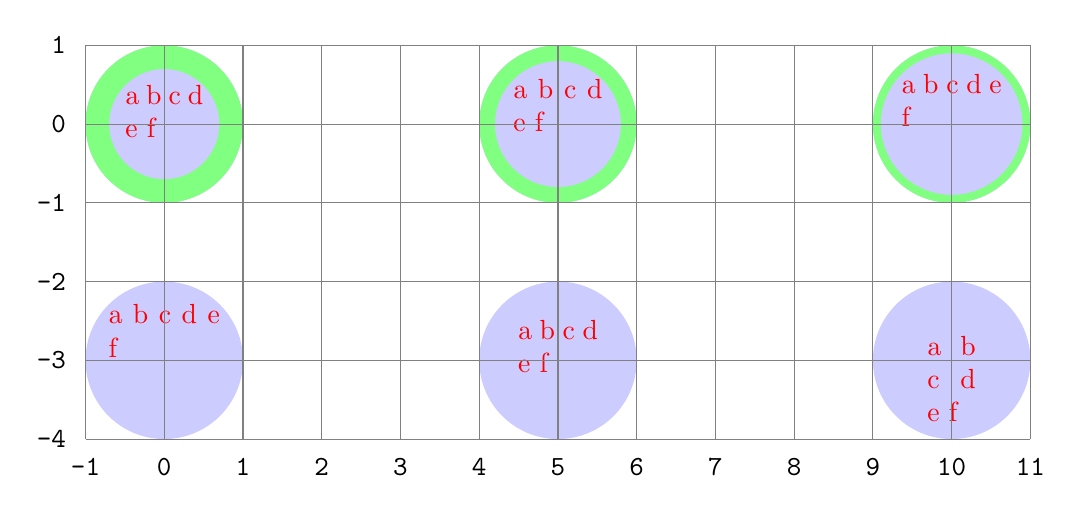
\begin{tikzpicture}
\fill[blue!20!white] (0.0, 0.0) circle (1);

\draw[line width=0.3cm,green!50!white] (0.0, 0.0)
circle (0.85);

\draw (0.0,0.0) node[color=red, inner sep=0cm] {
 
\begin{minipage}[t][0.99cm]{0.99cm}
a b c d e f
\end{minipage}

};\fill[blue!20!white] (5.0, 0.0) circle (1);

\draw[line width=0.2cm,green!50!white] (5.0, 0.0)
circle (0.9);

\draw (5.0,0.0) node[color=red, inner sep=0cm] {
 
\begin{minipage}[t][1.132cm]{1.132cm}
a b c d e f
\end{minipage}

};\fill[blue!20!white] (10.0, 0.0) circle (1);

\draw[line width=0.1cm,green!50!white] (10.0, 0.0)
circle (0.95);

\draw (10.0,0.0) node[color=red, inner sep=0cm] {
 
\begin{minipage}[t][1.273cm]{1.273cm}
a b c d e f
\end{minipage}

};\fill[blue!20!white] (0.0, -3.0) circle (1);

\draw (0.0,-3.0) node[color=red, inner sep=0cm] {
 
\begin{minipage}[t][1.414cm]{1.414cm}
a b c d e f
\end{minipage}

};\fill[blue!20!white] (5.0, -3.0) circle (1);

\draw (5.0,-3.0) node[color=red, inner sep=0.2cm] {
 
\begin{minipage}[t][1.014cm]{1.014cm}
a b c d e f
\end{minipage}

};\fill[blue!20!white] (10.0, -3.0) circle (1);

\draw (10.0,-3.0) node[color=red, inner sep=0.4cm] {
 
\begin{minipage}[t][0.614cm]{0.614cm}
a b c d e f
\end{minipage}

};\draw[gray] (-1.0,-4.0) -- (-1.0,1);
\draw[gray] (0.0,-4.0) -- (0.0,1);
\draw[gray] (1.0,-4.0) -- (1.0,1);
\draw[gray] (2.0,-4.0) -- (2.0,1);
\draw[gray] (3.0,-4.0) -- (3.0,1);
\draw[gray] (4.0,-4.0) -- (4.0,1);
\draw[gray] (5.0,-4.0) -- (5.0,1);
\draw[gray] (6.0,-4.0) -- (6.0,1);
\draw[gray] (7.0,-4.0) -- (7.0,1);
\draw[gray] (8.0,-4.0) -- (8.0,1);
\draw[gray] (9.0,-4.0) -- (9.0,1);
\draw[gray] (10.0,-4.0) -- (10.0,1);
\draw[gray] (11.0,-4.0) -- (11.0,1);
\draw[gray] (-1.0,-4.0) -- (11,-4.0);
\draw[gray] (-1.0,-3.0) -- (11,-3.0);
\draw[gray] (-1.0,-2.0) -- (11,-2.0);
\draw[gray] (-1.0,-1.0) -- (11,-1.0);
\draw[gray] (-1.0,0.0) -- (11,0.0);
\draw[gray] (-1.0,1.0) -- (11,1.0);
\draw(-1, -4) node [font=\ttfamily, label=below:{\texttt{-1}}] {};
\draw(0, -4) node [font=\ttfamily, label=below:{\texttt{0}}] {};
\draw(1, -4) node [font=\ttfamily, label=below:{\texttt{1}}] {};
\draw(2, -4) node [font=\ttfamily, label=below:{\texttt{2}}] {};
\draw(3, -4) node [font=\ttfamily, label=below:{\texttt{3}}] {};
\draw(4, -4) node [font=\ttfamily, label=below:{\texttt{4}}] {};
\draw(5, -4) node [font=\ttfamily, label=below:{\texttt{5}}] {};
\draw(6, -4) node [font=\ttfamily, label=below:{\texttt{6}}] {};
\draw(7, -4) node [font=\ttfamily, label=below:{\texttt{7}}] {};
\draw(8, -4) node [font=\ttfamily, label=below:{\texttt{8}}] {};
\draw(9, -4) node [font=\ttfamily, label=below:{\texttt{9}}] {};
\draw(10, -4) node [font=\ttfamily, label=below:{\texttt{10}}] {};
\draw(11, -4) node [font=\ttfamily, label=below:{\texttt{11}}] {};
\draw(-1, -4) node [font=\ttfamily, label=left:{\texttt{-4}}] {};
\draw(-1, -3) node [font=\ttfamily, label=left:{\texttt{-3}}] {};
\draw(-1, -2) node [font=\ttfamily, label=left:{\texttt{-2}}] {};
\draw(-1, -1) node [font=\ttfamily, label=left:{\texttt{-1}}] {};
\draw(-1, 0) node [font=\ttfamily, label=left:{\texttt{0}}] {};
\draw(-1, 1) node [font=\ttfamily, label=left:{\texttt{1}}] {};
\end{tikzpicture}

\end{center}

\end{document}
